\documentclass{beamer}
\usepackage[utf8]{inputenc}
\usepackage[spanish]{babel}
\usetheme{Warsaw}
\graphicspath{ {imagenes/} }
\spanishdecimal{.}

\title{Teorema de Bayes}
\subtitle{Probabilidad y Estadística}
\author{Joel C. Flores Escalante }
\date{Noviembre 2019}

\begin{document}

\begin{frame}
\titlepage
\end{frame}

\begin{frame}
\frametitle{Índice}
\tableofcontents
\end{frame}

%\begin{frame}
%\frametitle{Índice}
%\tableofcontents[pausesections]
%\end{frame}

\section{Introducción}
\subsection{Bayes}

\begin{frame}{Bayes}
    \begin{center}
     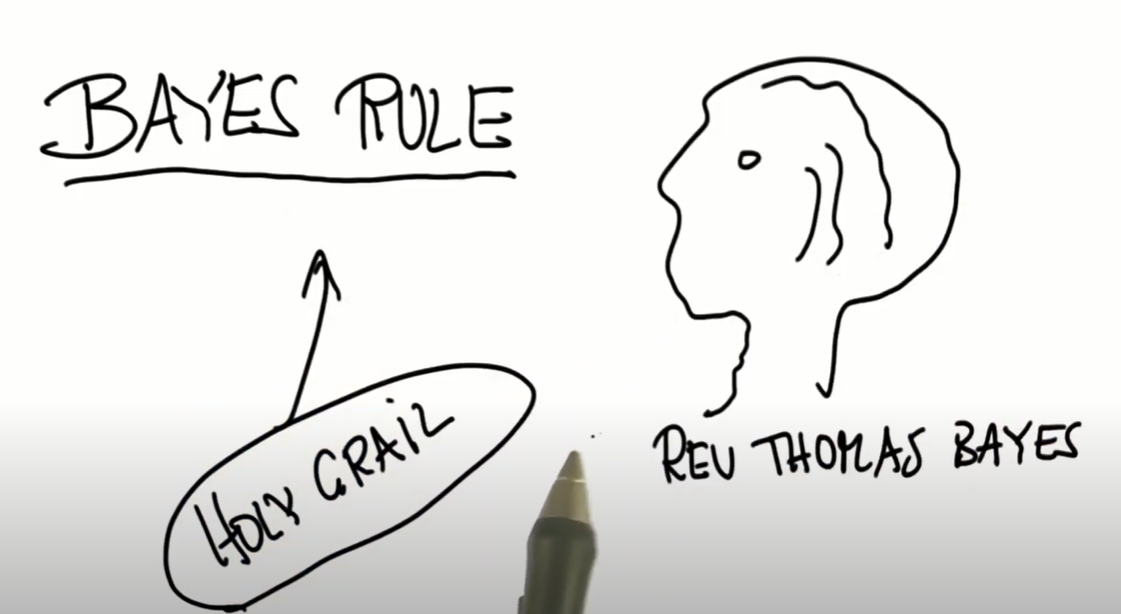
\includegraphics[scale=0.33]{br.png} 
     \end{center}
     \url{https://www.youtube.com/watch?v=CohZnkZMOxE}
\end{frame}

\subsection{Conocimiento previo}

\begin{frame}{Conocimiento previo}
     \begin{itemize}
         \item Probabilidad condicional
         \item Regla multiplicativa
         \item Principio de probabilidad total
         \item Árboles de probabilidad
     \end{itemize}
\end{frame}

\begin{frame}{Probabilidad condicional}
     \begin{itemize}
         \item[] $P(A|B) = \dfrac{P(A \cap B)}{P(B)}$
         \item \alert{o también:}
         \item[] $P(B|A) = \dfrac{P(B \cap A)}{P(A)}$
         
     \end{itemize}
\end{frame}

\begin{frame}{Regla multiplicativa}
\begin{itemize}
    \item La regla multiplicativa permite calcular la probabilidad de que dos eventos sucedan.
    \item[] $P(A|B) = \dfrac{P(A \cap B)}{P(A)}$
    \item[] $P(A \cap B) = P(A|B)P(A)$
    \item Dado que los eventos $(A \cap B)$ y $(B \cap A)$ son equivalentes, también se puede escribir: \item[] $P(A \cap B)=P(B \cap A)=P(B|A)P(B)$
    \item Es decir, no importa que evento se considere como A y cuál como B.
\end{itemize}
\end{frame}

\begin{frame}{Regla multiplicativa}
     \begin{itemize}
         \item \alert{Es decir:}
         \item[] $P(A \cap B) = P(A|B) P(B)$ 
         \item \alert{o también:}
         \item[] $P(B \cap A) = P(B|A) P(A)$ 
         \item \alert{Si} 
         \item[] $A\cap B = B \cap A$
         \item \alert{Entonces:}
         \item[] $P(A\cap B) = P(B \cap A)$
         \item[] $P(A\cap B)= P(A|B) P(B) = P(B|A) P(A)$
         \item[] $P(B\cap A)= P(B|A) P(A) = P(A|B) P(B)$
     \end{itemize}
\end{frame}

\begin{frame}{Principio de probabilidad total}
     \begin{center}
     
\includegraphics[scale=0.35]{ptotales1.png}
     \end{center}
\end{frame}

\begin{frame}{Principio de probabilidad total}
      \begin{center}
     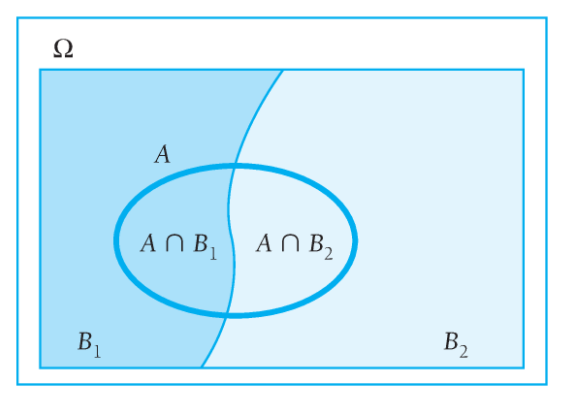
\includegraphics[scale=0.6]{ptotales2.png}
     \end{center}
\end{frame}

\begin{frame}{Principio de probabilidad total}
     \begin{itemize}
    \item \alert{Tenemos:}
       \item[] $A=(A \cap B_1) \cup (A \cap B_2)$
       \item[] $P(A)=P(A \cap B_1) + P(A \cap B_2)$
       \item \alert{Sustituyendo por la regla del producto:} 
       \item[] $P(A)=P(A|B_1)P(B_1) + P(A|B_2)P(B_2)$
   \end{itemize}
\end{frame}

\begin{frame}{Árboles de probabilidad}
      \begin{center}
     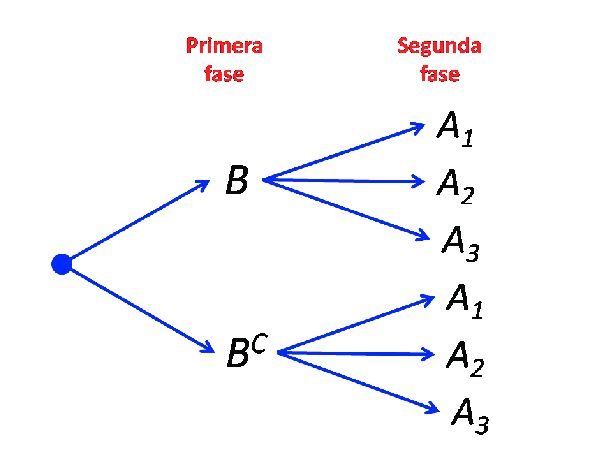
\includegraphics[scale=0.4]{Diagrama-de-arbol 2.png} 
     \end{center}
\end{frame}

\section{Teorema de Bayes}

\subsection{Versión simple}

\begin{frame}{Teorema de Bayes (versión simple)}
Ahora supongamos que se está interesado en la probabilidad condicional ``de un evento de la partición, digamos $B_1$ , dado que ocurre A", es decir, en $P(B_1|A)$, por definición:
\begin{itemize}
    
    \item[] $P(B_1|A)=\dfrac{P(B_1 \cap A)}{P(A)}$
    \item Usando la regla multiplicativa se sustituye $P(B_1 \cap A)$ por $P(B_1)P(A|B_1)$
    \item[] \alert{$P(B_1|A)= \dfrac{P(B_1)P(A|B_1)}{P(A)}$}
    \item Usando el principio de probabilidad total se sustituye $P(A)$ por $P(B_1)P(A|B_1) + P(B_2)P(A|B_2)$
    \item[] \alert{$P(B_1|A)= \dfrac{P(B_1)P(A|B_1)}{P(B_1)P(A|B_1) + P(B_2)P(A|B_2)}$}
\end{itemize}
\end{frame}

%\subsection{Ejemplo 1}

\begin{frame}{Ejemplo 1 }
En una compañía de seguros 30\% de los agentes de ventas son hombres y 70\% son mujeres. Se sabe que 10\% de los agentes hombres y 15\% de los agentes mujeres padecen estrés. Se elije una persona al azar de la población y se detecta que tiene estrés. ¿Cuál es la probabilidad que sea mujer?
\begin{itemize}
    \item[] Sabemos que:
    \item $B_1=$ ``Ser hombre" 
    \item $B_2=$ ``Ser mujer"
    \item E = ``tener estrés"
\end{itemize}
\end{frame}

\begin{frame}{Aplicación de la regla}
    \begin{itemize}
        \item[] $P(B_1)=0.3$
        \item[] $P(B_2)=0.7$
        \item[] $P(E|B_1)=0.1$
        \item[] $P(E|B_2)=0.15$
        \item[] $P(B_2|E)=\dfrac{P(B_2)P(E|B_2)}{P(B_1)P(E|B_1) + P(B_2)P(E|B_2)}$
        \item[] $P(B_2|E)=\dfrac{(0.7)(0.15)}{(0.3)(0.1)+(0.7)(0.15)}=\dfrac{0.105}{0.137}=\dfrac{7}{9}=0.777$
    \end{itemize}
\end{frame}

\begin{frame}{Árbol de probabilidad}
     \begin{center}
     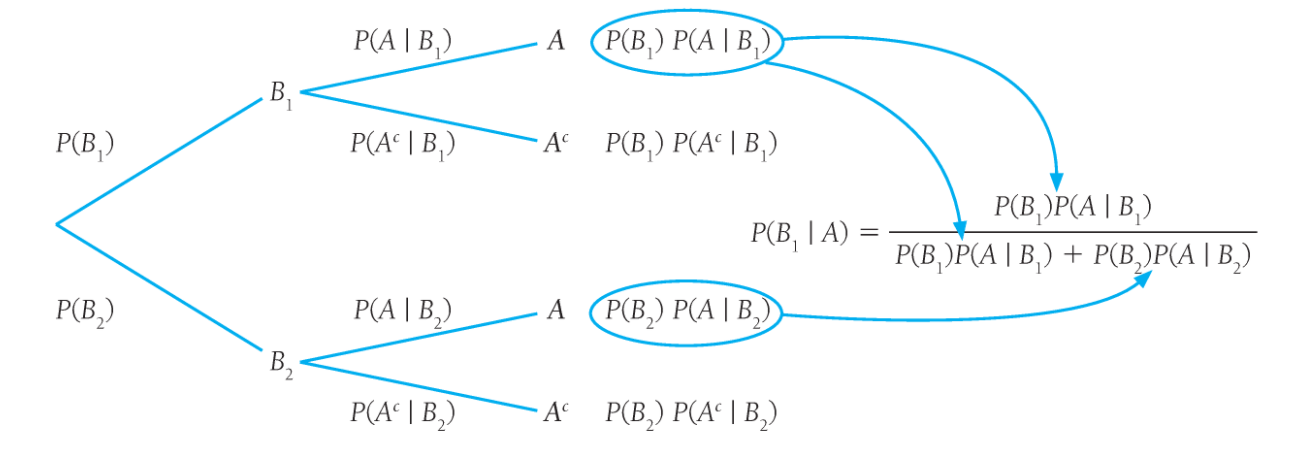
\includegraphics[scale=0.33]{diaEjemplo1.png} 
     \end{center}
\end{frame}

\subsection{Versión extendida}

\begin{frame}{Versión extendida}
\begin{itemize}
    \item[] $P(B_r|A)= \dfrac{P(B_r)P(A|B_r)}{\sum_{i=1}^k P(B_1 \cap A)}=\dfrac{P(B_r)P(A|B_r)}{\sum_{i=1}^k P(B_i)P(A|B_i)}$
\end{itemize}
\end{frame}

%\subsection{Ejemplo 2}
\begin{frame}{Ejemplo 2}
\begin{center}
    \includegraphics<1>[scale=0.34]{e1.png} 
    \includegraphics<2>[scale=0.34]{e2.png}
    \includegraphics<3>[scale=0.34]{e3.png}
    \includegraphics<4>[scale=0.34]{e4.png}
    \includegraphics<5>[scale=0.34]{e5.png}
    \includegraphics<6>[scale=0.34]{e6.png}
\end{center}
\end{frame}

\begin{frame}{Ejemplo 2}
\begin{itemize}
    \item[] $P(A|B)= \dfrac{P(B|A)P(A)}{P(B)}$
    \item[] $P(A|B)= \dfrac{P(B|A)P(A)}{P(B)}$
    \item[] $P(A|B)= \dfrac{P(B|A)P(A)}{P(E)(B|E) + P(P)(B|P) + P(A)(B|A)}$
\end{itemize}
\end{frame}

\begin{frame}{Aplicando la formula}
\begin{itemize}
    \item[] $P(A|B)= \dfrac{P(B|A)P(A)}{P(E)(B|E) + P(P)(B|P) + P(A)(B|A)}$
    \item[] $P(A|B)=\dfrac{(0.3)(0.3)}{(0.9)(0.2)+(0.6)(0.5)+(0.3)(0.3)}$
    \item[] $P(A|B)=\dfrac{0.09}{0.57}=0.157$
\end{itemize}
\end{frame}

\end{document}